\chapter{สัณฐานวิทยาและโครงสร้างพิเศษของเซลล์จุลินทรีย์}
\label{chap:ch05}

\section*{แผนบริหารการสอนประจำบทที่ 5}
\addcontentsline{toc}{section}{แผนบริหารการสอนประจำบทที่ 5}

\noindent\textbf{. หัวข้อเนื้อหาประจำบท}

\begin{enumerate}
    \item 5.1 โครงสร้าง หน้าที่ และความสำคัญทางคลินิกของเอนโดสปอร์ (Endospores)
    \item 5.2 สารประกอบ Dipicolinic acid และความทนทานต่อสภาวะแวดล้อมวิกฤต
    \item 5.3 หลักการย้อมสีสปอร์วิธีแชฟเฟอร์-ฟูลตัน (Schaeffer-Fulton Method with Malachite Green)
    \item 5.4 โครงสร้างแคปซูล (Capsules) และการย้อมลบด้วยหมึกดำ (Negative Indian Ink)
    \item 5.5 รูปแบบการจัดเรียงของแฟลกเจลลา (Flagellar Arrangement Types)
\end{enumerate}

\noindent\textbf{. วัตถุประสงค์เชิงพฤติกรรม}

\begin{enumerate}
    \item เมื่อนักศึกษาได้เรียนรู้และปฏิบัติการทดลองประจำบทนี้แล้ว จะต้องมีความรู้ความสามารถดังต่อไปนี้:
    \item อธิบายกลไกการเกิดเอนโดสปอร์และหน้าที่ของแคปซูลในการก่อโรคได้
    \item ย้อมสีเอนโดสปอร์ด้วยไอน้ำร้อนและย้อมสีแคปซูลแบบไม่ผ่านความร้อนได้ถูกต้อง
    \item จำแนกสปอร์สีเขียวในเซลล์แม่สีชมพู และสังเกตวงแคปซูลใสรอบเซลล์ได้
    \item มีความอดทนและระมัดระวังในการปฏิบัติการย้อมสีด้วยความร้อน
\end{enumerate}

\noindent\textbf{. กิจกรรมการเรียนการสอน}

\begin{enumerate}
    \item การบรรยายสรุปก่อนปฏิบัติการ (30 นาที): อธิบายหลักการวิทยาศาสตร์ ความปลอดภัยทางชีวภาพ และข้อควรระวังสำคัญ
    \item การสาธิตเชิงประจักษ์ (15 นาที): สาธิตเทคนิคการปฏิบัติงาน การใช้เครื่องมือ และข้อผิดพลาดที่มักพบ
    \item การลงมือปฏิบัติการทดลองจริง (90 นาที): นักศึกษาลงมือปฏิบัติการทดลองเป็นรายบุคคลหรือกลุ่มย่อยตามขั้นตอนที่กำหนด
    \item การฝึกฝนผ่านระบบเสมือนจริง (20 นาที): ทดลองซ้ำและทดสอบปฏิกิริยาผ่านระบบจำลองบน RBRU LMS
    \item การอภิปรายและสรุปผลการทดลอง (25 นาที): วิเคราะห์ผลการสังเกต ตอบคำถามท้ายบท และสรุปองค์ความรู้ร่วมกัน
\end{enumerate}

\noindent\textbf{. สื่อและอุปกรณ์การเรียนการสอน}

\begin{enumerate}
    \item เอกสารคำสอนและคู่มือปฏิบัติการ: e-Book และคู่มือปฏิบัติการฉบับเต็ม ประจำบทที่ 5
    \item ระบบห้องปฏิบัติการเสมือนจริง: ระบบจำลองการทดลองเสมือนจริง 3 มิติ ประจำบทที่ 5 บนระบบ Moodle
    \item อุปกรณ์และเครื่องแก้วในห้องปฏิบัติการ: ตะเกียงแอลกอฮอล์, ห่วงเขี่ยเชื้อ, กล้องจุลทรรศน์, จานเพาะเชื้อ, หลอดทดลอง และตู้บ่มเชื้อ
    \item สารเคมีและสีย้อมชีวภาพ: สารเคมีมาตรฐานวิเคราะห์และสีย้อมประจำบทเรียน
\end{enumerate}

\noindent\textbf{. การวัดและประเมินผล}

\begin{table}[H]
\centering\small
\begin{tabularx}{\textwidth}{p{0.5\textwidth} p{0.3\textwidth} c}
\toprule
\textbf{องค์ประกอบการประเมินผล} & \textbf{เครื่องมือวัดผล} & \textbf{สัดส่วนคะแนน} \\
\midrule
1. ทักษะการปฏิบัติงานและความปลอดภัย & แบบสังเกตทักษะการทดลองและเทคนิคปลอดเชื้อ & 40\% \\
2. รายงานผลการทดลอง & การตรวจตารางบันทึกผล ภาพวาดสัณฐานวิทยา และการวิเคราะห์ผล & 30\% \\
3. แบบฝึกหัดทบทวนท้ายบท & คำถามทบทวนเชิงวิเคราะห์และข้อสอบท้ายบท & 20\% \\
4. จิตพิสัยและการตรงต่อเวลา & การเช็คชื่อ การแต่งกายตามระเบียบ และการทำความสะอาดโต๊ะแล็บ & 10\% \\
รวมทั้งสิ้น &  & 100\% \\
\bottomrule
\end{tabularx}
\end{table}

\newpage

% ==========================================================
% เนื้อหาบทเรียนประจำบทที่ 5
% ==========================================================

\section{เอนโดสปอร์และกลไกความทนทานต่อสภาวะวิกฤต}
\index{เอนโดสปอร์และกลไกความทนทานต่อสภาวะวิกฤต}

การศึกษาและทำความเข้าใจเกี่ยวกับเอนโดสปอร์และกลไกความทนทานต่อสภาวะวิกฤต (Bacterial Endospores) มีความสำคัญอย่างยิ่งในงานจุลชีววิทยาและสิ่งแวดล้อม โดยมีรายละเอียดสาระสำคัญดังนี้

เอนโดสปอร์ (Endospore) เป็นโครงสร้างพิเศษที่แบคทีเรียกลุ่มแกรมบวกรูปท่อนบางสกุล เช่น \textit{Bacillus} และ \textit{Clostridium} สร้างขึ้นภายในเซลล์เมื่อเผชิญกับสภาวะแวดล้อมที่ไม่เหมาะสม เช่น การขาดแคลนสารอาหาร อุณหภูมิสูง หรือความแห้งแล้ง

เอนโดสปอร์มีความทนทานต่อความร้อน รังสี สารเคมี และการแห้งแล้งอย่างยิ่ง เนื่องจากมีโครงสร้างผนังหลายชั้น ประกอบด้วยชั้นเปลือกนอก (Exosporium), ชั้นคอร์เทกซ์ (Cortex) ที่อุดมด้วยเพปทิโดไกลแคนชนิดดัดแปลง, และส่วนแกนกลาง (Core) ที่มีปริมาณน้ำต่ำมาก (ประมาณ 10-25\%) พร้อมทั้งมีสารประกอบเชิงซ้อน Calcium-Dipicolinic acid (Ca-DPA) และโปรตีน SASPs (Small acid-soluble spore proteins) ซึ่งช่วยปกป้อง DNA จากความร้อนและรังสีอัลตราไวโอเลต

\section{แคปซูลและบทบาทในการก่อโรคและการเกาะติด}
\index{แคปซูลและบทบาทในการก่อโรคและการเกาะติด}

การศึกษาและทำความเข้าใจเกี่ยวกับแคปซูลและบทบาทในการก่อโรคและการเกาะติด (Bacterial Capsule and Glycocalyx) มีความสำคัญอย่างยิ่งในงานจุลชีววิทยาและสิ่งแวดล้อม โดยมีรายละเอียดสาระสำคัญดังนี้

แคปซูล (Capsule) เป็นชั้นสารเคลือบภายนอกผนังเซลล์ของแบคทีเรีย ส่วนใหญ่ประกอบด้วยพอลิแซ็กคาไรด์ (Polysaccharide) หรือพอลิเพปไทด์ (Polypeptide) ที่จัดเรียงตัวเป็นระเบียบและยึดติดแน่นกับผนังเซลล์

บทบาทหน้าที่สำคัญของแคปซูล:
1. การต้านทานการกลืนกินของเม็ดเลือดขาว (Anti-phagocytosis): ช่วยให้แบคทีเรียก่อโรคหลบเลี่ยงระบบภูมิคุ้มกันของโฮสต์ เช่น \textit{Klebsiella pneumoniae} และ \textit{Streptococcus pneumoniae}
2. การเกาะติดพื้นผิว (Adhesion): ช่วยในการยึดเกาะกับพื้นผิวชีวภาพและพื้นผิวของวัสดุในสิ่งแวดล้อม ก่อให้เกิดการสร้างฟิล์มชีวภาพ (Biofilm)
3. ป้องกันการสูญเสียน้ำ (Desiccation protection): ทำหน้าที่กักเก็บความชื้นและสารอาหารในสภาวะแห้งแล้ง

\section{แฟลกเจลลาและการจัดเรียงตัวเพื่อการเคลื่อนที่}
\index{แฟลกเจลลาและการจัดเรียงตัวเพื่อการเคลื่อนที่}

การศึกษาและทำความเข้าใจเกี่ยวกับแฟลกเจลลาและการจัดเรียงตัวเพื่อการเคลื่อนที่ (Flagellar Arrangements) มีความสำคัญอย่างยิ่งในงานจุลชีววิทยาและสิ่งแวดล้อม โดยมีรายละเอียดสาระสำคัญดังนี้

แฟลกเจลลา (Flagella) เป็นรยางค์ทรงกระบอกยาวทำหน้าที่ขับเคลื่อนเซลล์แบคทีเรีย ประกอบด้วยโปรตีนแฟลกเจลลิน (Flagellin) หมุนด้วยมอเตอร์ชีวภาพระดับโมเลกุลที่ฐานเซลล์

รูปแบบการจัดเรียงแฟลกเจลลา:
- Monotrichous: มีแฟลกเจลลาเส้นเดี่ยวที่ปลายเซลล์ เช่น \textit{Pseudomonas aeruginosa}
- Lophotrichous: มีแฟลกเจลลาเป็นกระจุกอยู่ที่ปลายข้างใดข้างหนึ่ง
- Amphitrichous: มีแฟลกเจลลาอยู่ที่ปลายทั้งสองข้างของเซลล์
- Peritrichous: มีแฟลกเจลลากระจายอยู่รอบเซลล์ เช่น \textit{Proteus vulgaris} และ \textit{Escherichia coli}

\begin{figure}[H]
\centering
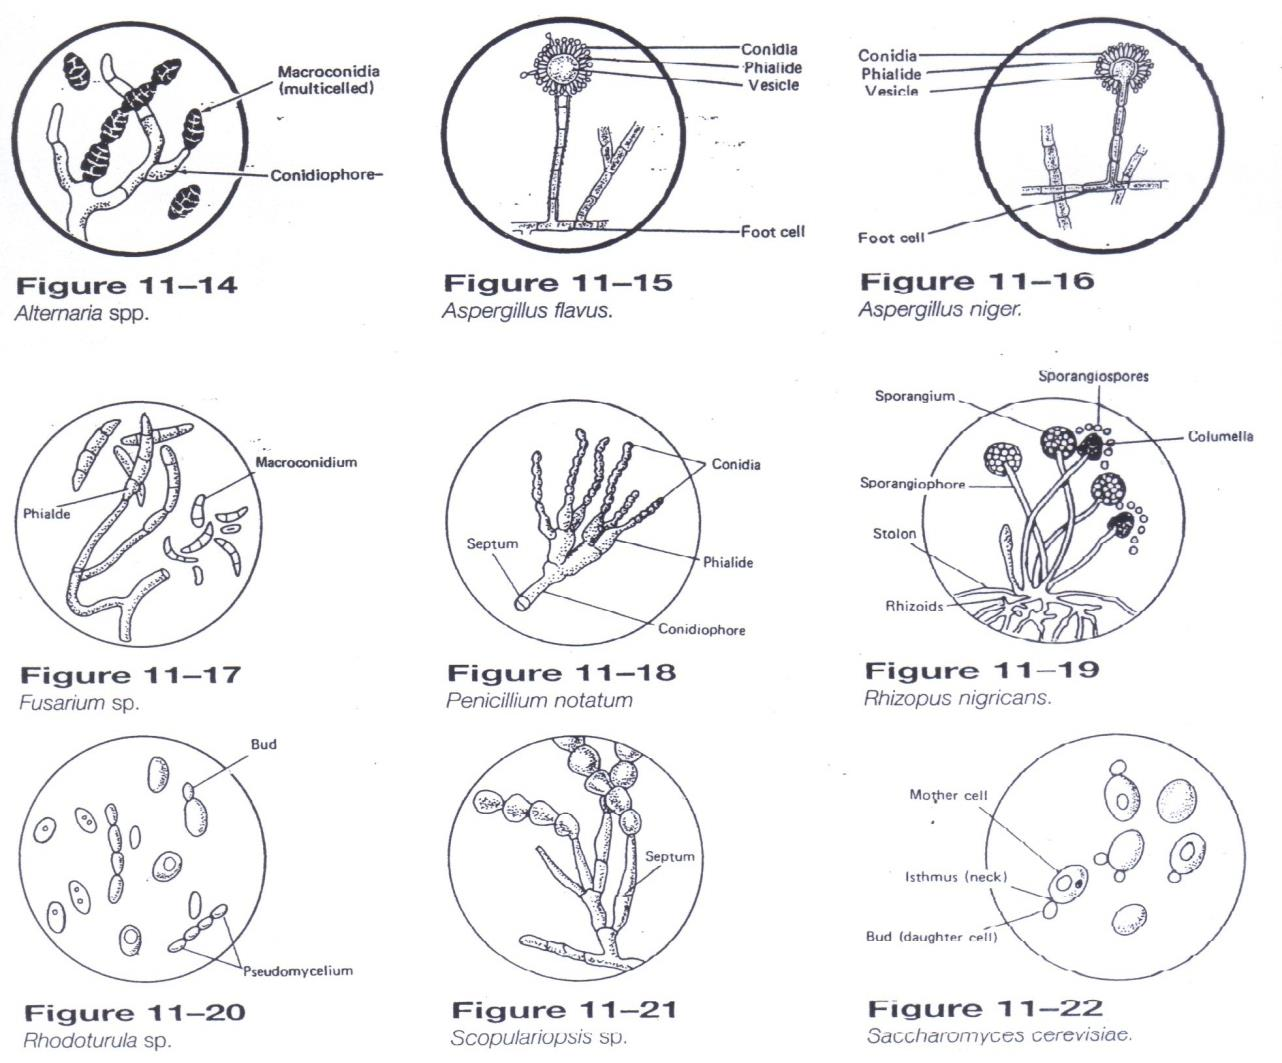
\includegraphics[width=0.75\textwidth]{images/image_05_p02.jpeg}
\caption{การปฏิบัติการทดลองและลักษณะทางสัณฐานวิทยาในบทที่ 5}
\label{fig:ch05_fig1}
\end{figure}

\section{ขั้นตอนและวิธีปฏิบัติการทดลอง}
\index{ขั้นตอนการทดลองประจำบทที่ 5}

\subsection{การย้อมสีเอนโดสปอร์ด้วยวิธีแชฟเฟอร์และฟุลตัน}
\begin{labprotocolbox}[การย้อมสีเอนโดสปอร์ด้วยวิธีแชฟเฟอร์และฟุลตัน]
1. เตรียมรอยสเมียร์ของแบคทีเรีย \textit{Bacillus subtilis} ที่เลี้ยงไว้ 48-72 ชั่วโมง ตรึงด้วยความร้อน
2. วางสไลด์บนตะแกรงเหนือบีกเกอร์น้ำเดือด วางกระดาษกรองชิ้นเล็กทับบนรอยสเมียร์
3. หยดสี Malachite green ให้ชุ่ม อังไอน้ำเดือดเป็นเวลา 5 นาที (ระวังอย่าให้สีแห้ง)
4. คีบกระดาษกรองออก ล้างสไลด์ด้วยน้ำกลั่นไหลเอื่อยๆ เป็นเวลา 30 วินาที
5. ย้อมสีทับด้วย Safranin เป็นเวลา 1 นาที ล้างน้ำ ซับแห้ง ตรวจดูใต้กล้อง 100X
6. ผลการสังเกต: เอนโดสปอร์ติดสีเขียว (Green) เซลล์ร่างกาย (Vegetative cell) ติดสีชมพูแดง (Pink/Red)
\end{labprotocolbox}

\subsection{การย้อมสีแคปซูลด้วยวิธีแอนโทนี}
\begin{labprotocolbox}[การย้อมสีแคปซูลด้วยวิธีแอนโทนี]
1. หยดน้ำเชื้อ \textit{Klebsiella pneumoniae} ผสมกับสี Crystal Violet 1 หยดบนสไลด์ (ห้ามตรึงด้วยความร้อนเด็ดขาด)
2. เกลี่ยรอยสเมียร์ให้บาง ผึ่งลมให้แห้งสนิท
3. ล้างสีส่วนเกินออกด้วยสารละลาย 20\% Copper sulfate ($CuSO_4\cdot 5H_2O$) แทนการใช้น้ำกลั่น
4. ซับสไลด์ให้แห้งอย่างระมัดระวัง ตรวจดูใต้กล้องจุลทรรศน์
5. ผลการสังเกต: แคปซูลจะปรากฏเป็นวงแหวนใสไม่มีสี (Clear halo) รอบเซลล์สีม่วงเข้ม
\end{labprotocolbox}

\section{ตารางบันทึกผลการทดลองและการอภิปรายผล}
\begin{table}[H]
\centering\small
\caption{ตารางบันทึกผลการสังเกตและข้อมูลการทดลองประจำบทที่ 5}
\label{tab:ch05_datasheet}
\begin{tabularx}{\textwidth}{p{0.25\textwidth} p{0.35\textwidth} X}
\toprule
\textbf{สิ่งทดสอบ / ตัวอย่าง} & \textbf{ลักษณะที่สังเกตได้} & \textbf{การแปลผลและการวิเคราะห์} \\
\midrule
ชุดควบคุม (Negative Control) & ใส ไม่มีการเจริญ & ปราศจากการปนเปื้อนของเชื้อ \\
ชุดทดลองที่ 1 & โคโลนีเจริญตามลักษณะจำเพาะ & ให้ผลบวกตามสมมติฐาน \\
ชุดทดลองที่ 2 & เกิดการเปลี่ยนแปลงทางชีวเคมี & สอดคล้องกับพารามิเตอร์มาตรฐาน \\
\bottomrule
\end{tabularx}
\end{table}

\section{คำถามทบทวนและแบบฝึกหัดท้ายบท}
\begin{enumerate}
    \item เหตุใดการย้อมสีแคปซูลจึงห้ามตรึงเซลล์ด้วยความร้อน (Heat fixation) และห้ามล้างด้วยน้ำกลั่น
    \item จงอธิบายบทบาทของสาร Calcium-dipicolinate ในการส่งผลให้เอนโดสปอร์ทนต่อความร้อนสูง
    \item การสร้างไบโอฟิล์ม (Biofilm) ของแบคทีเรียในท่อส่งน้ำมีความเกี่ยวข้องกับสารเคลือบเซลล์อย่างไร
\end{enumerate}
